\documentclass{article}
\usepackage{graphicx}
\usepackage{amsmath}
\usepackage[colorlinks=true, linkcolor=blue, citecolor=red]{hyperref}

\title{The three layer model}
\author{Bernardo S. Mendoza and Sean M. Anderson}

\begin{document}
\maketitle

\section{\texorpdfstring{$\mathcal{R}_{pP}$}{Rpp}}

For practicality, we wish to review only the main results. From your document,
we make the following observations:

\begin{enumerate}
\item Eq. (3) of your notes is now replaced by:
\begin{equation}\label{m81}
\begin{split}
r_{pP} &=
\sin\theta\epsilon_{b}(2\omega)
\Big[
  \sin^2\theta\epsilon^2_{b}(\omega)\chi_{\perp\perp\perp}
+ k^2_{zb}(\omega)\epsilon^2_{\ell}(\omega)\chi_{\perp\parallel\parallel}
\Big]\\
&- \epsilon_{\ell}(\omega)\epsilon_{\ell}(2\omega)
   k_{zb}(\omega)k_{zb}(2\omega)
\Big[
  2\sin\theta\epsilon_{b}(\omega)\chi_{\parallel\parallel\perp}
+ k_{zb}(\omega)\epsilon_{\ell}(\omega)
\chi_{\parallel\parallel\parallel}\cos(3\phi) 
\Big],
\end{split}
\end{equation}
where the sign on the $\chi_{\parallel\parallel\parallel}$ term has been derived
correctly, and is now negative as you pointed out in your notes.

\item Two layer limit: as it turns out, to go from the above expression to the
two layer limit, it is a little bit more subtle. The reason being that in the
papers by Sipe, Moss, and van Driel \cite{sipePRB87}, and Mizrahi and Sipe
\cite{mizrahiJOSA88} the second-harmonic polarization is put on top of the
surface in the vacuum region, and the fundamental field is evaluated inside the
bulk region.

In order to reduce the three layer model $r_{pP}$ of Eq. \eqref{m81} to that of
Refs. \cite{mizrahiJOSA88} and \cite{sipePRB87},  we take the $2\omega$
radiations factors for vacuum by taking $\ell=v$, thus
$\epsilon_{\ell}(2\omega)=1$,
%$T^{\ell v}_{p}=1$, $T^{\ell b}_{p}=T^{vb}_{p}$, 
and the fundamental field inside medium $b$ by taking $\ell=b$, thus
$\epsilon_{\ell}(\omega)=\epsilon_{b}(\omega)$
%$t^{v\ell}_{p}=t^{vb}_{p}$, and $t^{\ell b}_{p}=1$
. With these choices,
\begin{equation}\label{m82}
\begin{split}
r_{pP}
&= \sin\theta\epsilon_{b}(2\omega)
\Big[
\sin^2\theta\chi_{\perp\perp\perp} + k^{2}_{zb}(\omega)
\chi_{\perp\parallel\parallel}
\Big]\\
&- k_{zb}(\omega)k_{zb}(2\omega)
\Big[
2\sin\theta\chi_{\parallel\parallel\perp} + k_{zb}(\omega)
\chi_{\parallel\parallel\parallel}\cos(3\phi) 
\Big].
\end{split}
\end{equation}
Please note that the $\epsilon^{2}_{b}(\omega)$ that is factorized from Eq.
\eqref{m81} is included into the Fresnel factors shown in Eq. (1) of your notes
that we do omit here for brevity.

We remark that Eq. \eqref{m82} is identical to what one gets from completing the
algebra from either Refs. \cite{sipePRB87} and \cite{mizrahiJOSA88} which both
yield the same result. This is in contrast to Eq. 6 of your notes since that
equation has an extra $\epsilon_{b}(2\omega)$ factor multiplying the
$\chi_{\perp\parallel\parallel}$ term.

In summary, these results are consistent when derived from the three layer
model, when derived directly from Ref. \cite{mizrahiJOSA88}, and when derived
directly from Ref. \cite{sipePRB87}, and that is to say that the two layer model
considers the nonlinear polarization on top of the surface in the vacuum region,
and the fundamental field in the bulk region. When these considerations are
taken into account, the three layer model reduces appropriately to the two layer
model.

\item Having clarified the previous points, the three layer model is now capable
of representing the following five cases:
\begin{description}
\item[Case 1] The three layer model where $\mathcal{P}(2\omega)$ is taken in the
small layer below the surface ($\ell$) characterized by
$\epsilon_{\ell}(\omega)$ and the fundamental fields are evaluated in the same
layer.
\item[Case 2] The two layer model where $\mathcal{P}(2\omega)$ is taken in the
vacuum region above the surface ($v$) characterized by $\epsilon_{v}(\omega) =
1$ and the fundamental fields are evaluated in the bulk region with
$\epsilon_{b}(\omega)$. We remark that this is the standard model used in the
literature, Refs. \cite{sipePRB87} and \cite{mizrahiJOSA88}.
\end{description}
We compare these two models in Fig. \ref{3layervs2layer} with the experiment for
$\mathcal{R}_{pP}$. As can be seen from the figure, the two layer model compares
more favorably with the experimental results, while the three layer model does
not reproduce the E$_{2}$ correctly. The intensity of both is higher than the
experimental value.

\begin{figure}[t]
\centering
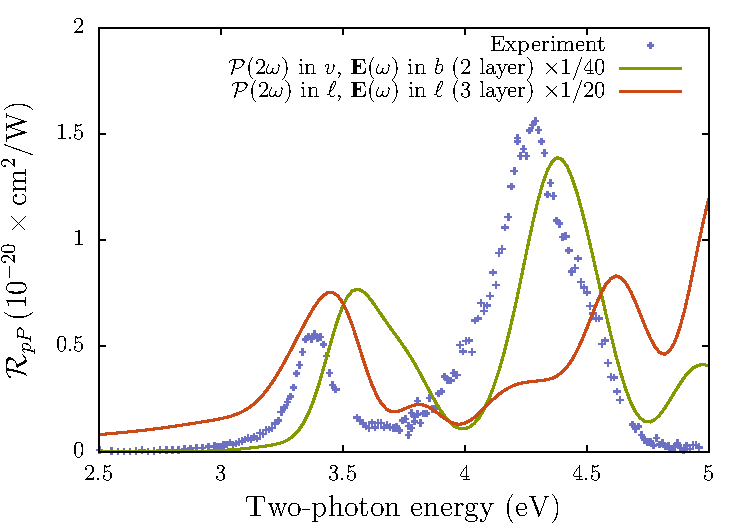
\includegraphics[width=0.75\textwidth]{figures/rpp-3vs2layer}
\caption{Comparison between the three and two layer models and experiment.}
\label{3layervs2layer}
\end{figure}

The remaining cases are when
\begin{description}
\item[Case 3] $\mathcal{P}(2\omega)$ is taken in the vacuum region above the
surface ($v$) characterized by $\epsilon_{v}(\omega) = 1$ and the fundamental
fields are also evaluated in the same region.
\item[Case 4] $\mathcal{P}(2\omega)$ is taken in the small layer region below
the surface ($\ell$) characterized by $\epsilon_{\ell}(\omega)$ and the
fundamental fields are evaluated in the bulk region with $\epsilon_{b}(\omega)$.
\item[Case 5] $\mathcal{P}(2\omega)$ is taken in the bulk region ($b$)
characterized by $\epsilon_{b}(\omega)$ and the fundamental fields are also
evaluated in the same region.
\end{description}
We compare these three cases in Fig. \ref{comparison} with the experiment for
$\mathcal{R}_{pP}$. As can be seen from the figure, the first two cases
yield a similar lineshape where E$_{1}$ is not well represented and the
intensity of both is 7 and 6 orders of magnitude higher than the experimental
value, respectively. The last scenario gives a lineshape where E$_{1}$ is well
represented but E$_{2}$ is incorrectly repdroduced. However, intensity for this
case is much closer to the experimental value.

\begin{figure}[t]
\centering
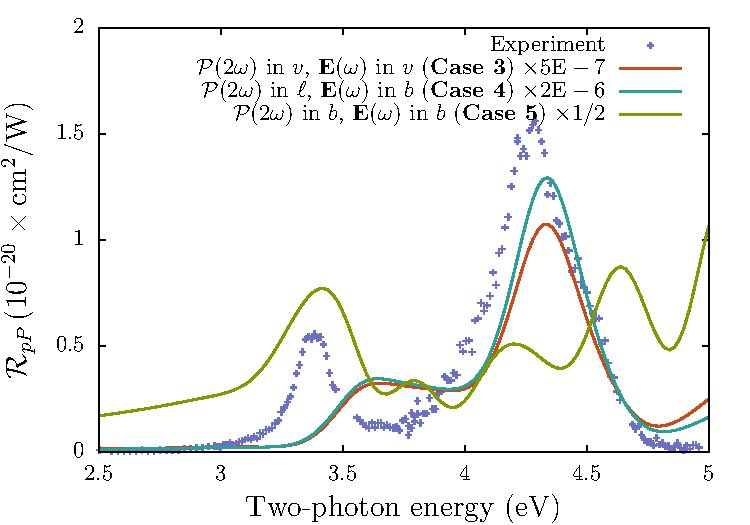
\includegraphics[width=0.75\textwidth]{figures/rpp-comparison}
\caption{Comparison between the remaining cases for $\mathcal{R}_{pP}$ and
experiment.}
\label{comparison}
\end{figure}
\end{enumerate}

Therefore, we may conclude that the two layer model, where
$\mathcal{P}(2\omega)$ is taken in the vacuum region above the surface ($v$)
characterized by $\epsilon_{v}(\omega) = 1$ and the fundamental fields are
evaluated in the bulk region with $\epsilon_{b}(\omega)$, is the best model for
$\mathcal{R}_{pP}$.

\section{\texorpdfstring{$\mathcal{R}_{pS}$}{RpS}}

For $R_{pS}(2\omega)$ we now have
\begin{equation}\label{eq:rps}
r_{pS}
= -\epsilon^{2}_{\ell}(\omega)k^{2}_{zb}(\omega)
\chi_{\parallel\parallel\parallel}\sin3\phi.
\end{equation} 
In order to reduce the above result to that of Refs. \cite{sipePRB87} and
\cite{mizrahiJOSA88} (two layer model), we take the $2\omega$ radiations factors
for vacuum by taking $\ell=v$, thus $\epsilon_{\ell}(2\omega)=1$, and the
fundamental field inside medium $b$ by taking $\ell=b$, thus
$\epsilon_{\ell}(\omega)=\epsilon_{b}(\omega)$. With these choices,
\begin{equation*}
r_{pS} = -k^{2}_{zb}(\omega)\chi_{\parallel\parallel\parallel}\sin3\phi.
\end{equation*} 
Please note that the $\epsilon^{2}_{b}(\omega)$ of Eq. \eqref{eq:rps} is
included into the Fresnel factors that we omit here for brevity. In Fig.
\ref{rps} we show the comparison between the three layer and two layer models
and experiment. Except for the intensity which is different, the lineshape is
very similar between the two. This is understandable since it is only
proportional to $\chi_{\parallel\parallel\parallel}$.

\begin{figure}[t]
\centering
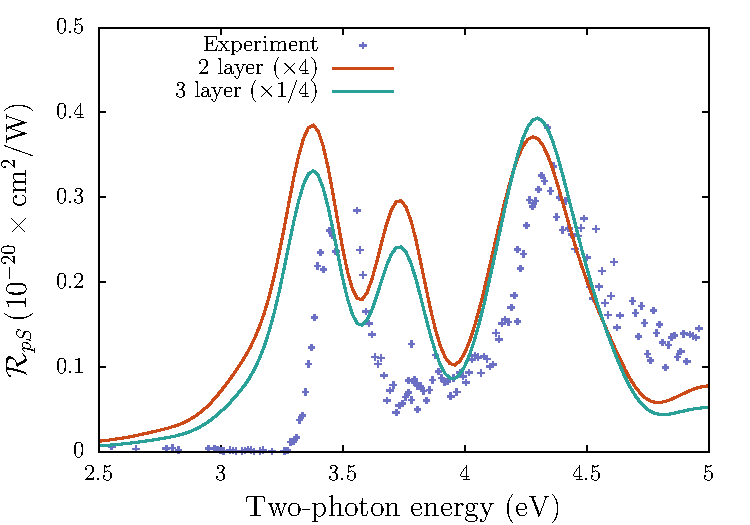
\includegraphics[width=0.75\textwidth]{figures/rps}
\caption{Comparison between the three layer and two layer models with
experiment for $\mathcal{R}_{pS}$.}
\label{rps}
\end{figure}

\section{\texorpdfstring{$\mathcal{R}_{sP}$}{RsP}}

For $R_{sP}(2\omega)$ we have
\begin{equation}
r_{sP}
= \sin\theta\epsilon_{b}(2\omega)\chi_{\perp\parallel\parallel}
+ \epsilon_{\ell}(2\omega)k_{zb}(2\omega)
  \chi_{\parallel\parallel\parallel}\cos3\phi.
\end{equation}
In order to reduce above result to that of Refs. \cite{sipePRB87} and
\cite{mizrahiJOSA88} (two layer model), we take the $2\omega$ radiations factors
for vacuum by taking $\ell=v$, thus $\epsilon_{\ell}(2\omega)=1$, and the
fundamental field inside medium $b$ by taking $\ell=b$, thus
$\epsilon_{\ell}(\omega)=\epsilon_{b}(\omega)$. With these choices,
\begin{equation*}
r_{sP} = \sin\theta\epsilon_{b}(2\omega)\chi_{\perp\parallel\parallel}
+ k_{zb}(2\omega)\chi_{\parallel\parallel\parallel}\cos3\phi.
\end{equation*} 
In Fig. \ref{rsp} we show the comparison between the three layer and two layer
models and experiment. The intensity of the two layer model is one order of
magnitude larger than that of the three layer model. The lineshape is similar
between the two, with the two layer model producing a more prominent E$_{2}$
peak. Since, for the azimuthal angle used ($\phi = 30$) the contribution from
the $\chi_{\parallel\parallel\parallel}$ term is zero, both lineshapes are quite
similar as they only depend on $\chi_{\perp\parallel\parallel}$

\begin{figure}[t]
\centering
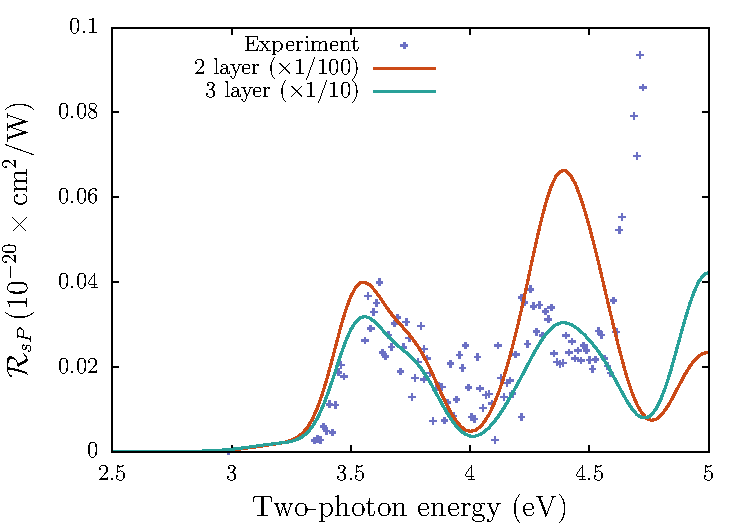
\includegraphics[width=0.75\textwidth]{figures/rsp}
\caption{Comparison between the three layer and two layer models with
experiment for $\mathcal{R}_{sP}$.}
\label{rsp}
\end{figure}


\section{Conclusions}

What we conclude after this analysis is that the two layer model (\textbf{Case
2}) is more appropriate to represent $\mathcal{R}_{iF}$ in general. Therefore,
we propose to only use this model and leave the three layer model (\textbf{Case
1}) and \textbf{Cases 3}, \textbf{4}, and \textbf{5} out of the manuscript and
only present the two layer model.

So, if you agree let us know and we will proceed to change the manuscript
accordingly for your next revision!


\bibliographystyle{unsrt}
\bibliography{/Users/sma/Dropbox/docs/academics/master}

\end{document}
